\chapter{Introducción al problema}

En este documento se describirá el proceso de confección de una metaheurística basada en un algoritmo genético para encontrar una solución al \textit{Maximum Diversity Problem}.

\section{Definición del problema}
El Maximum Diversity Problem (MDP) Problem consiste en, dado un conjunto de elementos, obtener el subconjunto en el que la diversidad de los elementos sea máxima. Esto es, dado un conjunto $N$ con cardinalidad $|N| = n$, obtener un subconjunto $M \subset N$, con cardinalidad $|M| = m$ y $m < n$ en el que se maximice la diversidad de sus elementos.

La función de diversidad se puede definir tal que:
\begin{equation}
    MD(x) = \sum^{n-1}_{i=0} \sum^{n}_{j=i+1} D_{ij}x_ix_j
\label{max-diversity}
\end{equation}

donde la solución es un número, que determina la diversidad de los elementos elegidos.

$D$ es una matriz de distancias que asocia la distancia de dos elementos del conjunto $N$, de forma que $D_{ij}$ determina la distancia entre el elemento $i$ y el elemento $j$ en el conjunto $N$.

$x$ es una solución posible, que se compone de $n$ elementos donde $x_i \in \{0, 1\}$, es decir, un vector binario. Este vector indica los índices de los elementos del conjunto $N$ que estamos tomando como posible combinación. De esta forma, la cardinalidad de $m$, se calcula como: 

\begin{equation}
    m = \sum_{i=0}^n x_i 
    \label{eq:sum_m}
\end{equation}

lo que nos dice el número de 1 que hay en el vector.

El problema se resume así a calcular qué combinación $x$ ofrece una diversidad mayor. Atendiendo a la ecuación \ref{max-diversity} vemos que el cálculo se sustenta sobre la formación del vector $x$. Al multiplicar $D_{ij}$ por $x_i$ y $x_j$, si alguno de ellos fuera 0, el producto se anula. Solo nos quedamos con aquellos índices en los que ambos sean 1, y el resultado del producto es la distancia entre estos dos elementos (que no necesariamente es conmutativa). Esto nos deja con un vector de distancias cuya suma debemos maximizar.


Como vemos, calcular esto no es una tarea fácil para un número arbitrario de $n$ o de $m$. Para dar un poco de perspectiva, el espacio de soluciones de un ejemplo con $n = 500$ y $m = 50$ es de $2.31 \times 10^{69}$. Se puede observar que el espacio de búsqueda es totalmente inabarcable, siendo este ejemplo uno considerado \textit{mediano}. Puede verse una evolución del crecimiento del espacio de búsqueda en la figura \ref{fig:binom}.



\begin{figure}[h]
    \centering
    
    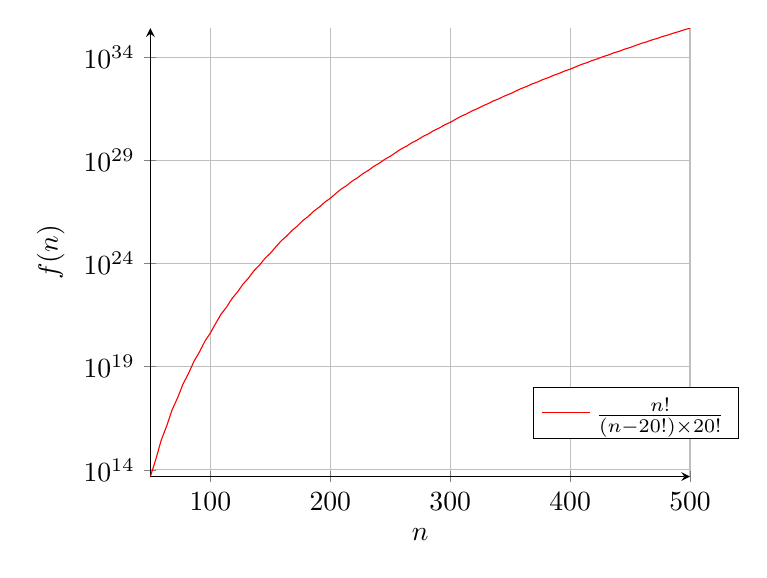
\begin{tikzpicture}
        \centering
        \begin{axis}[
            axis lines = left,
            xlabel = $n$,
            ylabel = {$f(n)$},
            ymode = log,
            grid = major,
            legend style = {at={(0.9,0.2)},
            anchor=north}
        ]
        %Below the red parabola is defined
        \addplot [
            domain=50:500, 
            samples=100, 
            color=red
        ]
        {x! / ((x - 20)! * 20!)};
        \addlegendentry{$\frac{n!}{(n-20!) \times 20!}$}
        
        \end{axis}
        \end{tikzpicture}
    
        \caption{Evolución del crecimiento del espacio de búsqueda en función de $n$, suponiendo que $m = 20$}
        \label{fig:binom}
    
    \end{figure}


\chapter{Detalles de la implementación}

Describiremos en este capítulo las diferentes consideraciones tomadas de cara a la implementación del algoritmo genético, así como el cálculo de la diversidad de las soluciones.

\section{Consideraciones previas}
Antes de empezar con la descripción de la metaheurística en sí, debemos ser capaces de, dada una potencial solución, calcular su diversidad. Además, debemos ser capaces de cerciorarnos de que dicha solución es válida, es decir, tiene exactamente $m$ unos.

\subsection{Formato de la solución}
Un requisito que presenta nuestro problema es el valor de $m$, que corresponde al número de unos que presenta nuestra solución, o lo que se traduce a exactamente cuál es la mayor diversidad que podemos encontrar en $m$ elementos dada una matriz de distancias $D$.

Para ello, se ha confeccionado una función \jesitt{shape\_solution} que recibe una solución y garantiza que esto es así. Consta de dos bucles while que preguntan por el número de unos (véase la ecuación \ref{eq:sum_m})


\cite{GRASP}